% !TeX program = xelatex
% !TeX encoding = UTF-8 Unicode
% !BIB program = biber

\documentclass{relatorio}

\title{Is Software Debloating Effective? - A comparative study}
\addauthor{Sumit Lahiri}
\addauthor{Amit Kumar Sharma}
\setsubject{Analysis Study \& Comparision of Software Debloating}

\preamble{}
\addbibresource{bibliothek.bib}

\begin{document}
	
	% !TeX root = document.tex
% !TeX encoding = UTF-8 Unicode

\IEEEtitleabstractindextext{%
	\begin{abstract}
		What is Program Debloating? What is Program Debloating? What is Program Debloating? What is Program Debloating? What is Program Debloating? 
		What is Program Debloating? What is Program Debloating? What is Program Debloating? What is Program Debloating? 
		What is Program Debloating? What is Program Debloating? What is Program Debloating? What is Program Debloating? What is Program Debloating? What is Program Debloating? 
		What is Program Debloating? What is Program Debloating? What is Program Debloating? 
		What is Program Debloating? What is Program Debloating? What is Program Debloating? What is Program Debloating? What is Program Debloating? What is Program Debloating? 
		What is Program Debloating? What is Program Debloating? What is Program Debloating? What is Program Debloating? What is Program Debloating? What is Program Debloating? What is Program Debloating? What is Program Debloating? What is Program Debloating? What is Program Debloating? What is Program Debloating? What is Program Debloating? What is Program Debloating? What is Program Debloating? What is Program Debloating? What is Program Debloating? What is Program Debloating? 
	\end{abstract}
	
	\begin{IEEEkeywords}
		Software Debloating, Software Engineering, Delta Debugging
	\end{IEEEkeywords}
}

	\maketitle{}
	
	\section{Tools}%
	\label{Tools}
	
	Program debloating techniques. Program deblaoting techniques rogram debloating techniques. Program deblaoting techniques
	rogram debloating techniques. Program deblaoting techniquesrogram debloating techniques. Program deblaoting techniques
	rogram debloating techniques. Program deblaoting techniques rogram debloating techniques. Program deblaoting techniques
	rogram debloating techniques. Program deblaoting techniques 
	rogram debloating techniques. Program deblaoting techniquesrogram debloating techniques. Program deblaoting techniques
	rogram debloating techniques. Program deblaoting techniques
	
	Program debloating techniques. Program deblaoting techniques rogram debloating techniques. Program deblaoting techniques
	rogram debloating techniques. Program deblaoting techniquesrogram debloating techniques. Program deblaoting techniques
	rogram debloating techniques. Program deblaoting techniques rogram debloating techniques. Program deblaoting techniques
	rogram debloating techniques. Program deblaoting techniques 
	rogram debloating techniques. Program deblaoting techniquesrogram debloating techniques. Program deblaoting techniques
	rogram debloating techniques. Program deblaoting techniques
	\begin{figure}[H]
		\centering
		\captionsetup{justification=centering}
		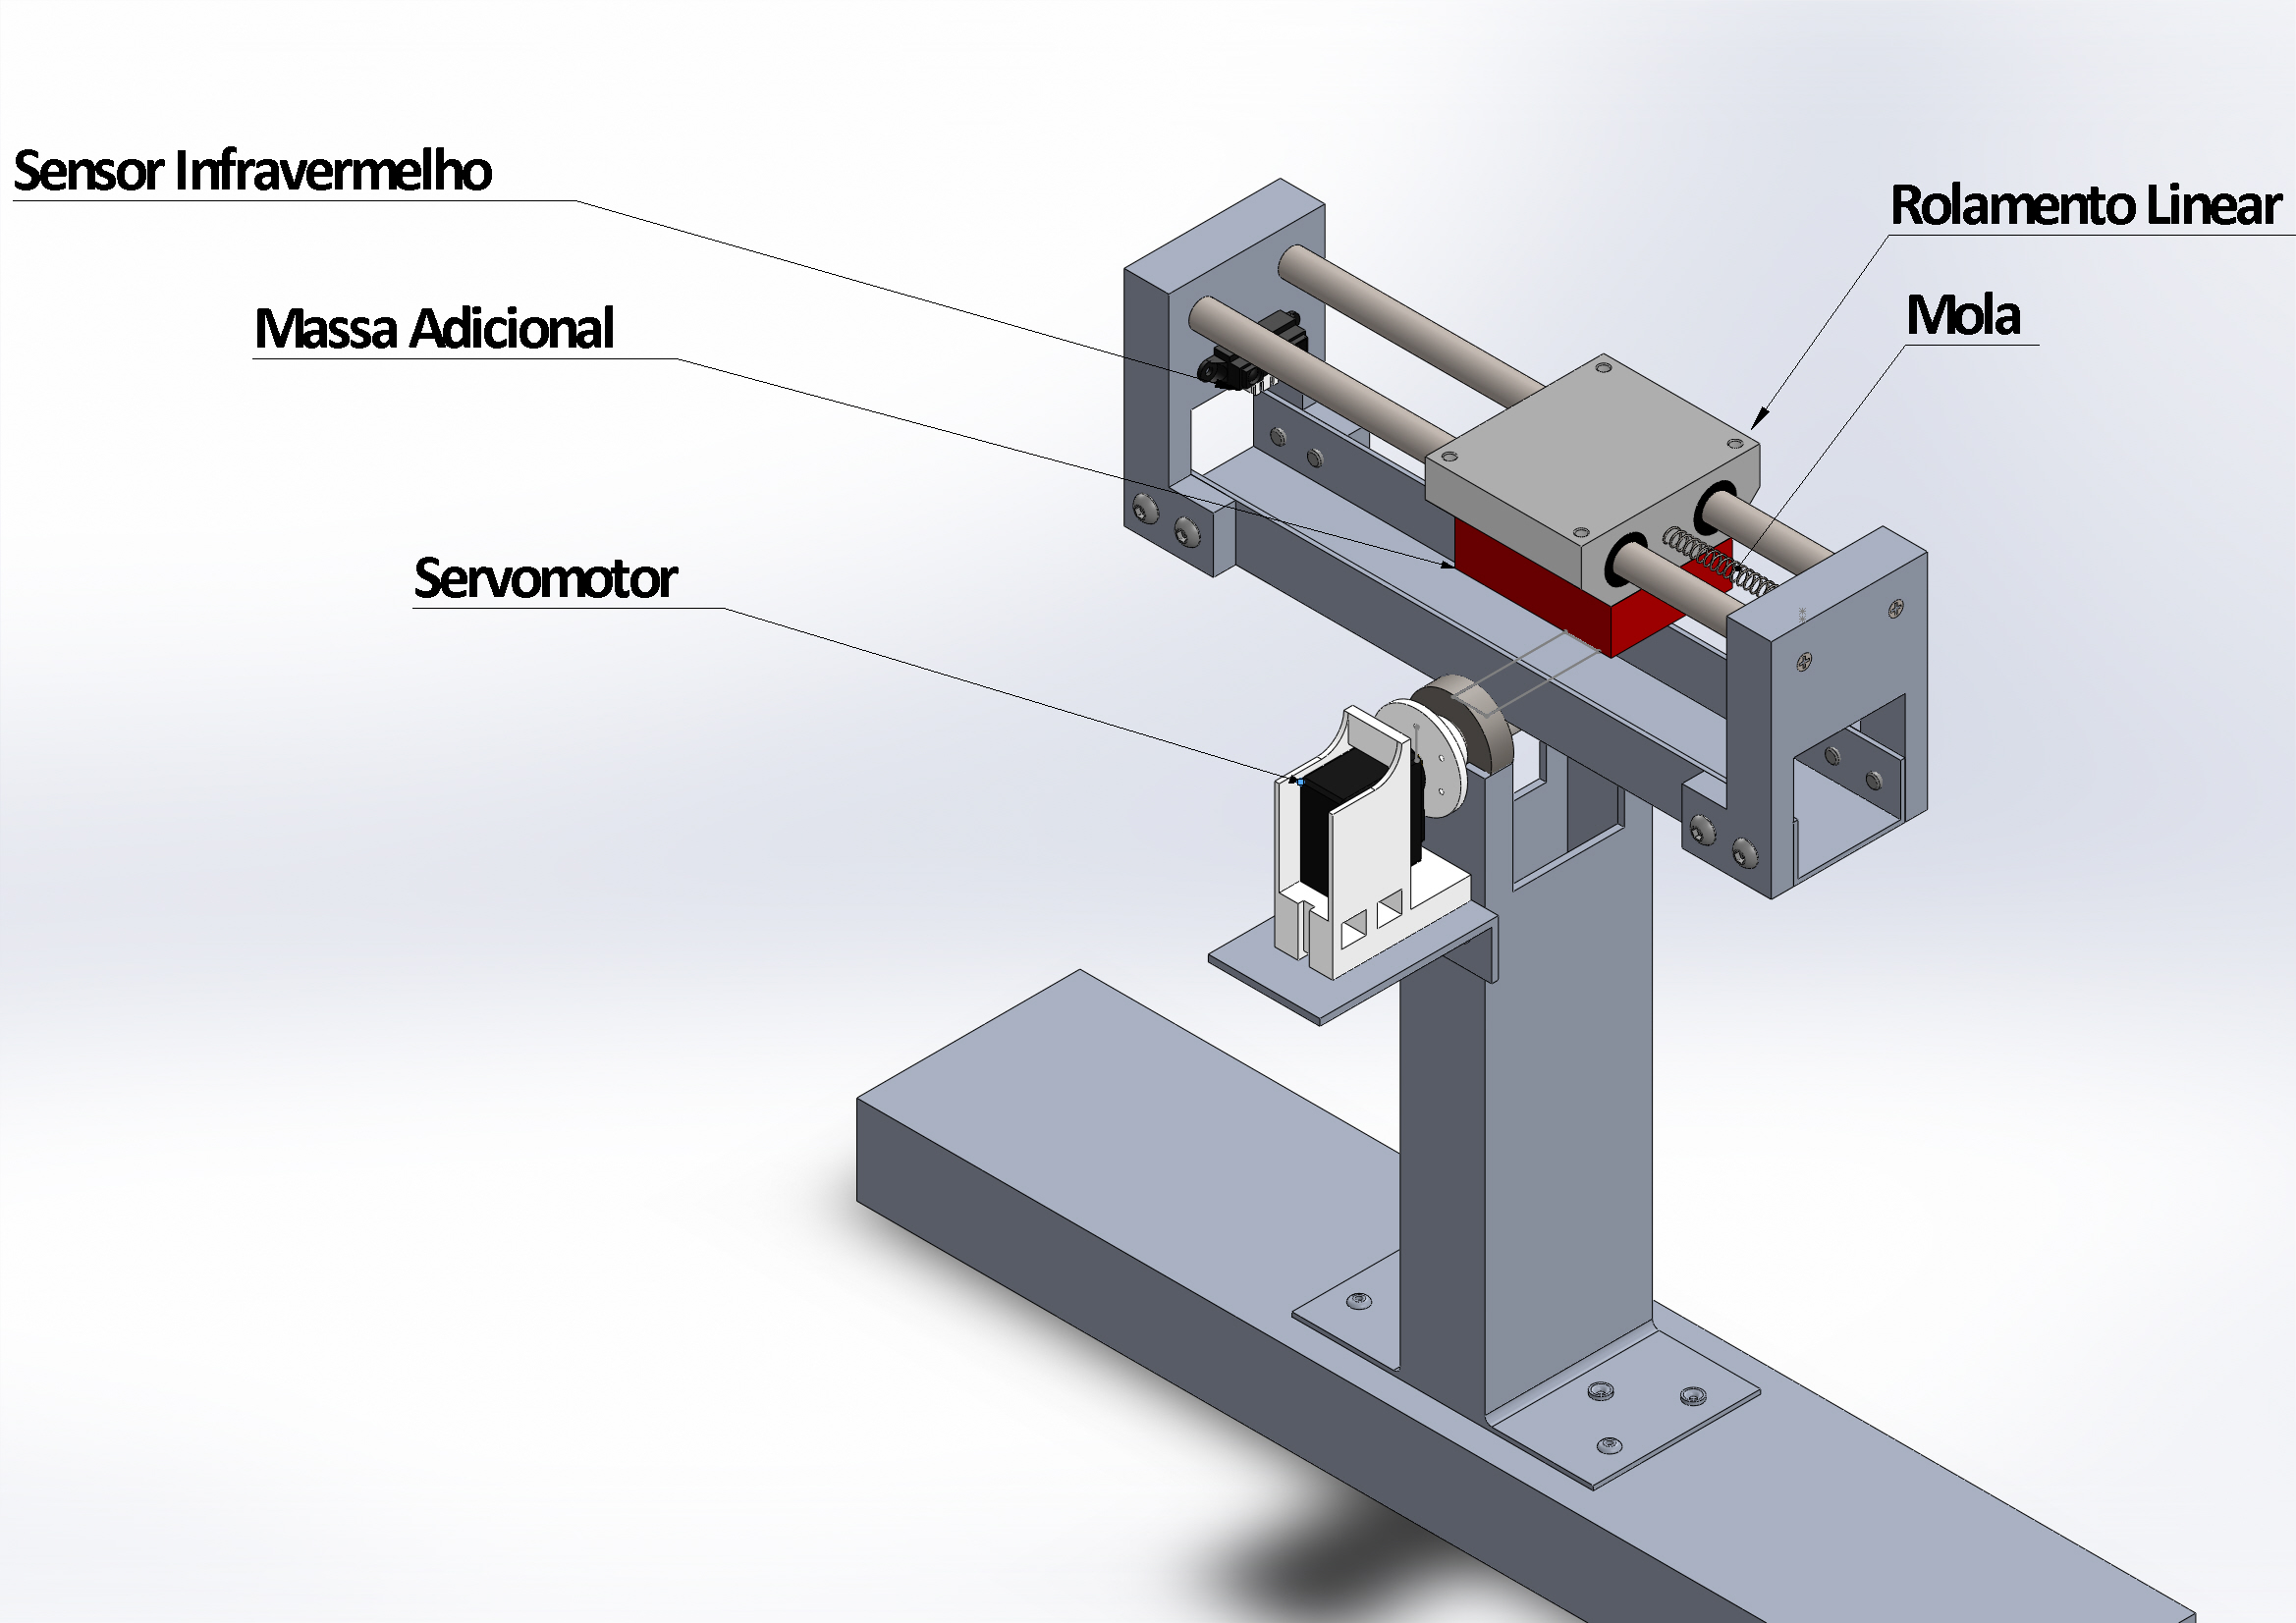
\includegraphics[width=0.8\linewidth]{imgs/planta}
		\caption{Sistema massa-mola em plano inclinado}%
		\label{fig:plant}
		\centering
		\captionsetup{justification=centering}
		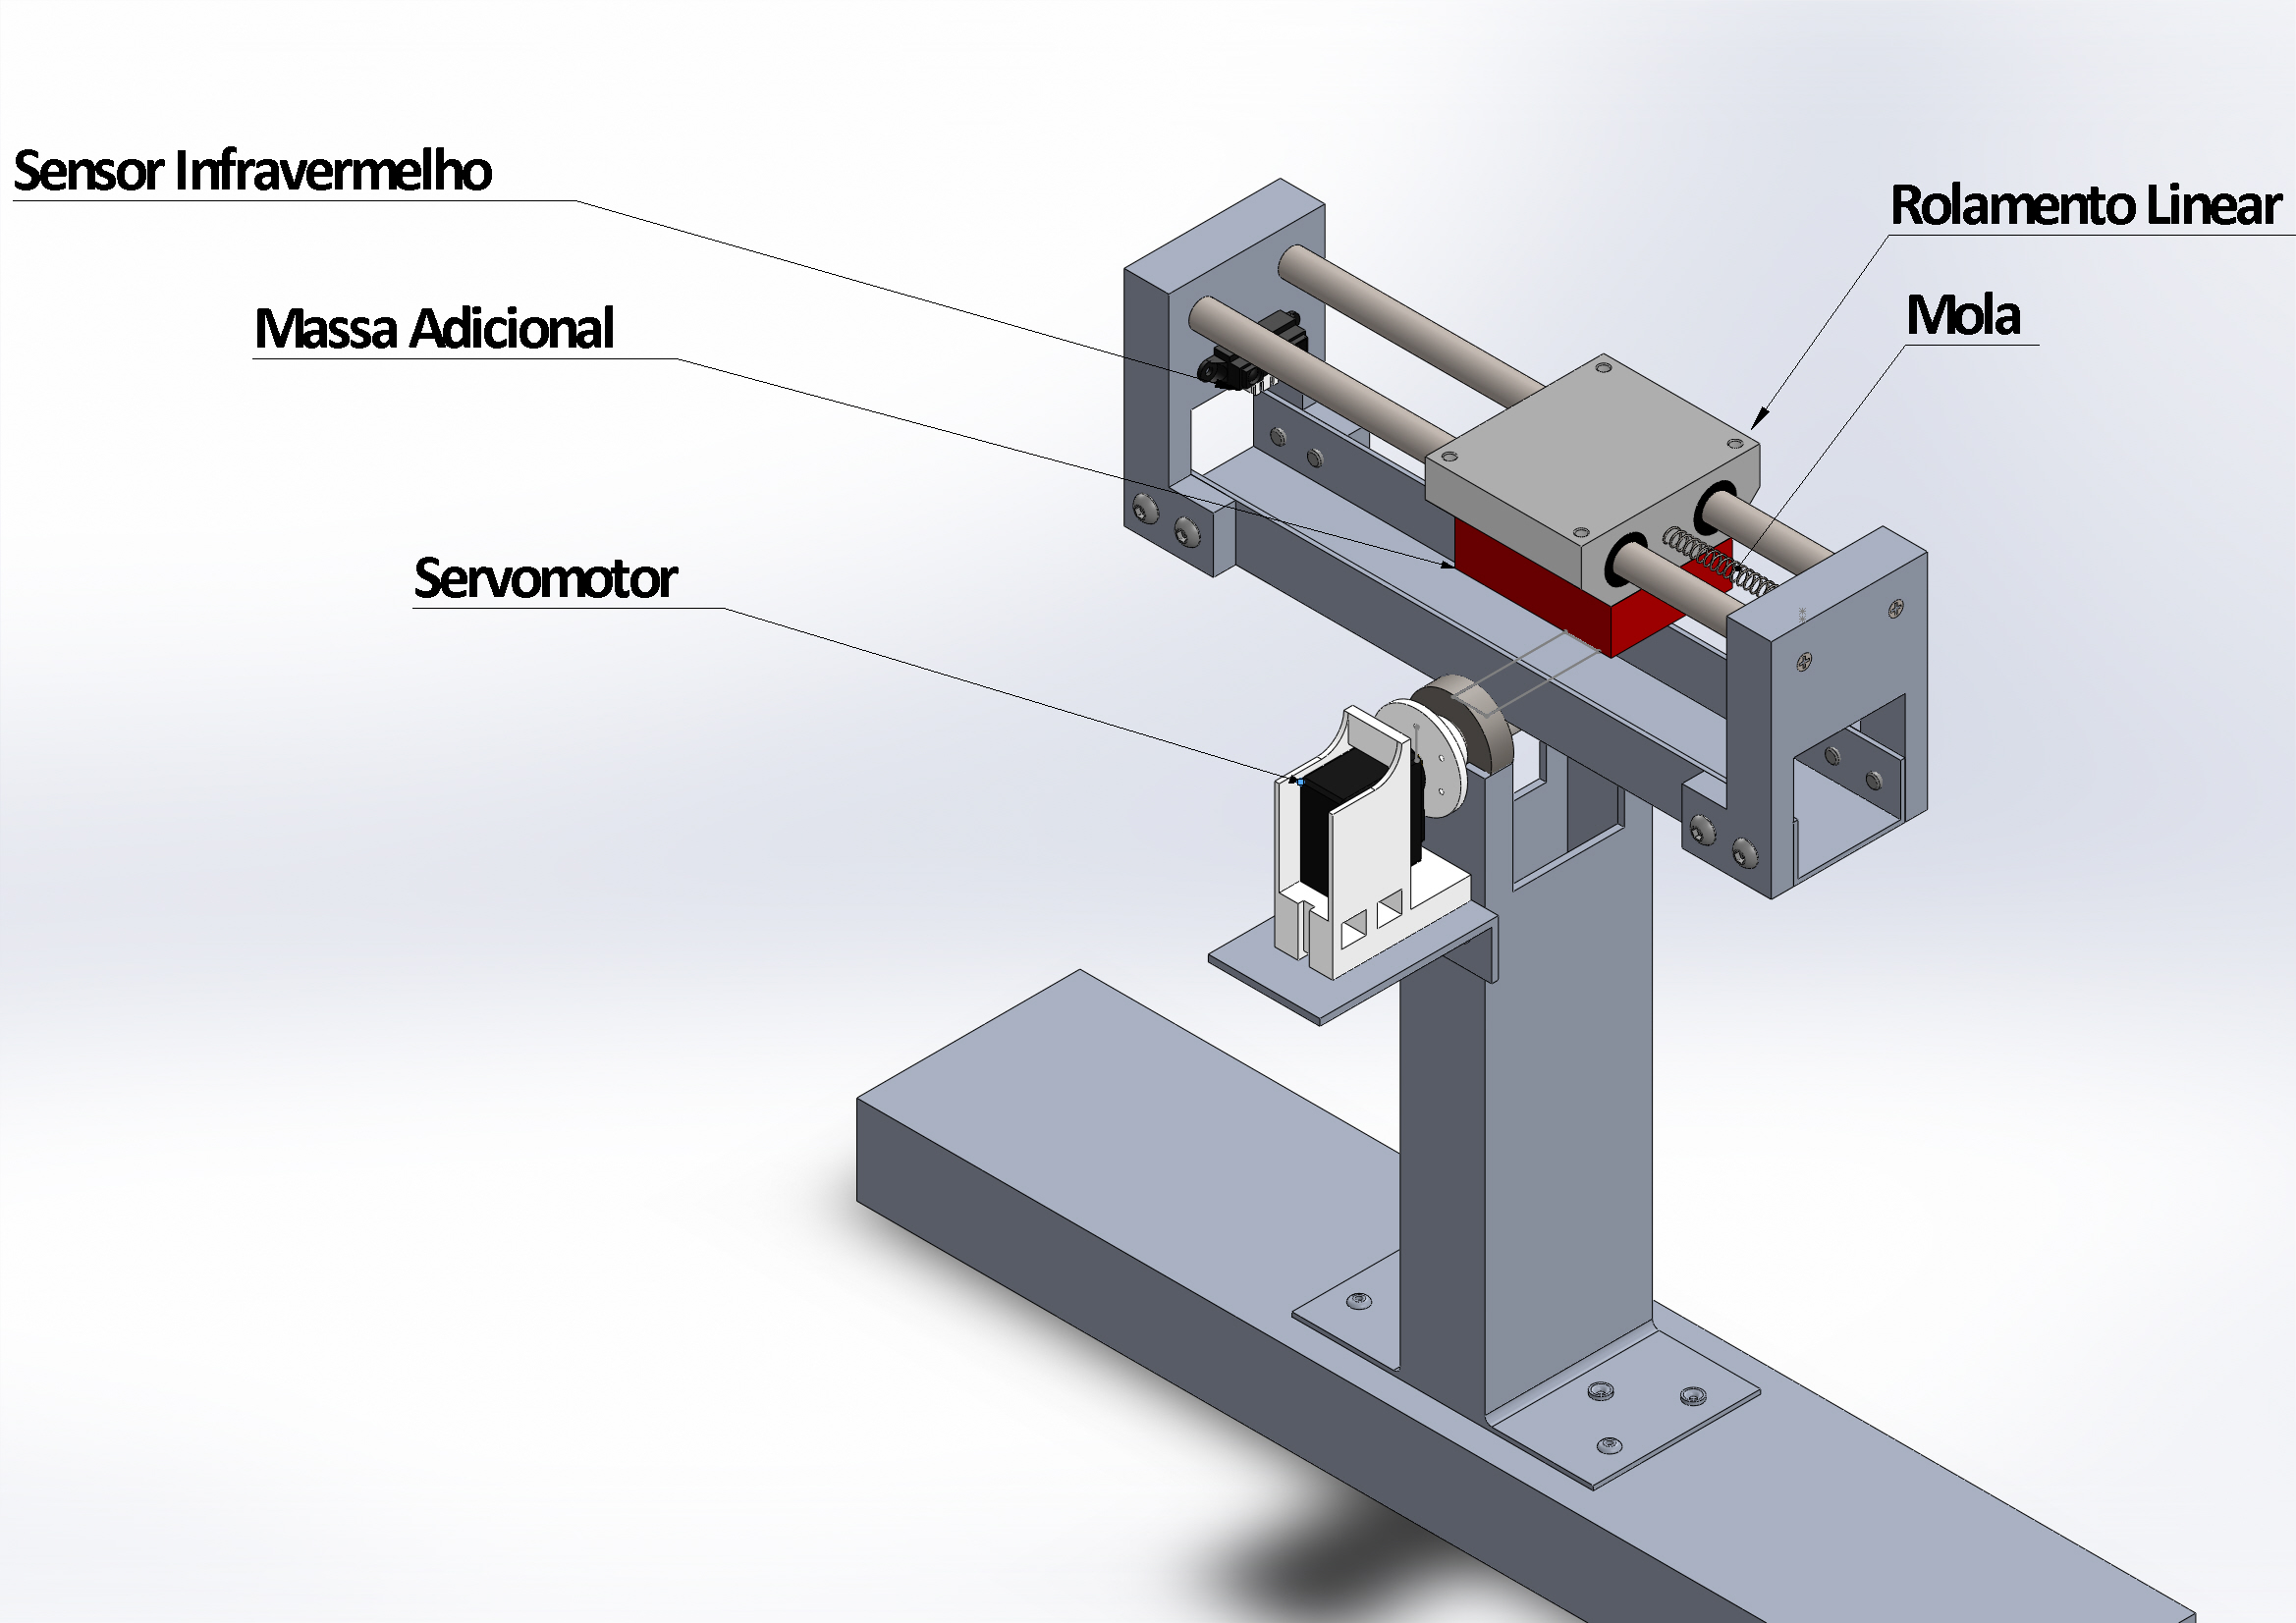
\includegraphics[width=0.8\linewidth]{imgs/planta}
		\caption{Sistema massa-mola em plano inclinado}%
		\label{fig:plant}
		\centering
		\captionsetup{justification=centering}
		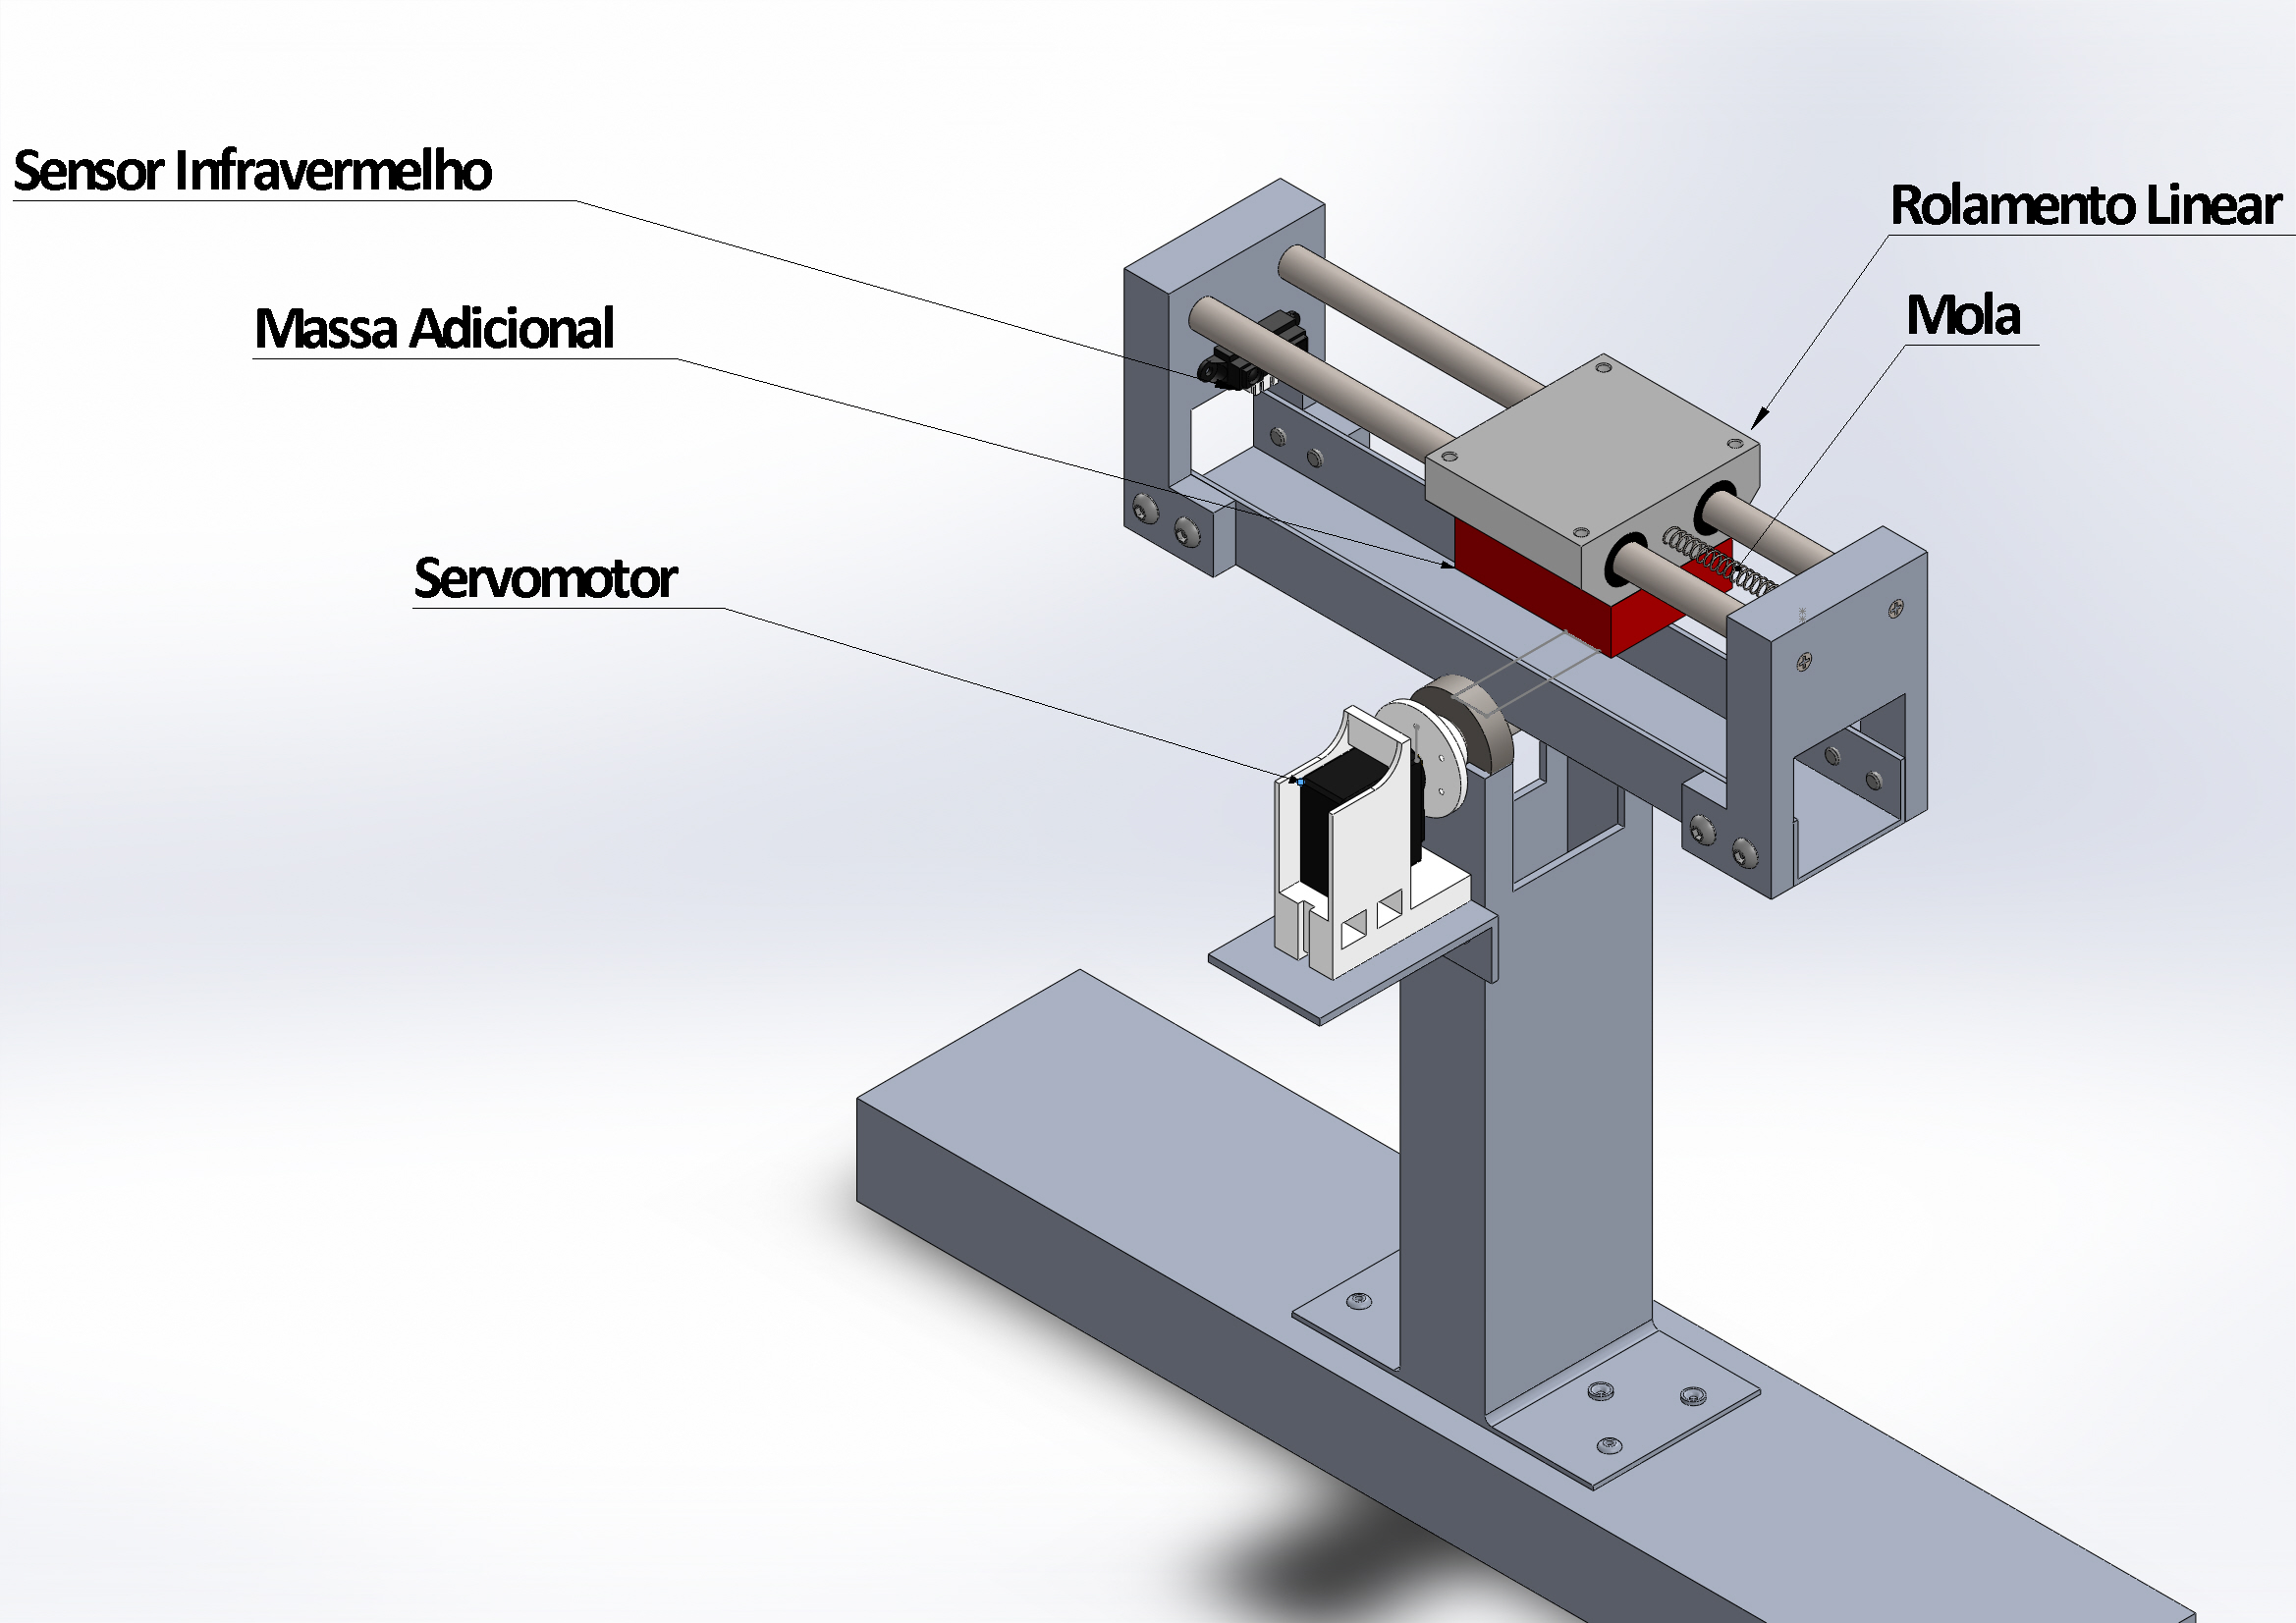
\includegraphics[width=0.8\linewidth]{imgs/planta}
		\caption{Sistema massa-mola em plano inclinado}%
		\label{fig:plant}
		\centering
		\captionsetup{justification=centering}
		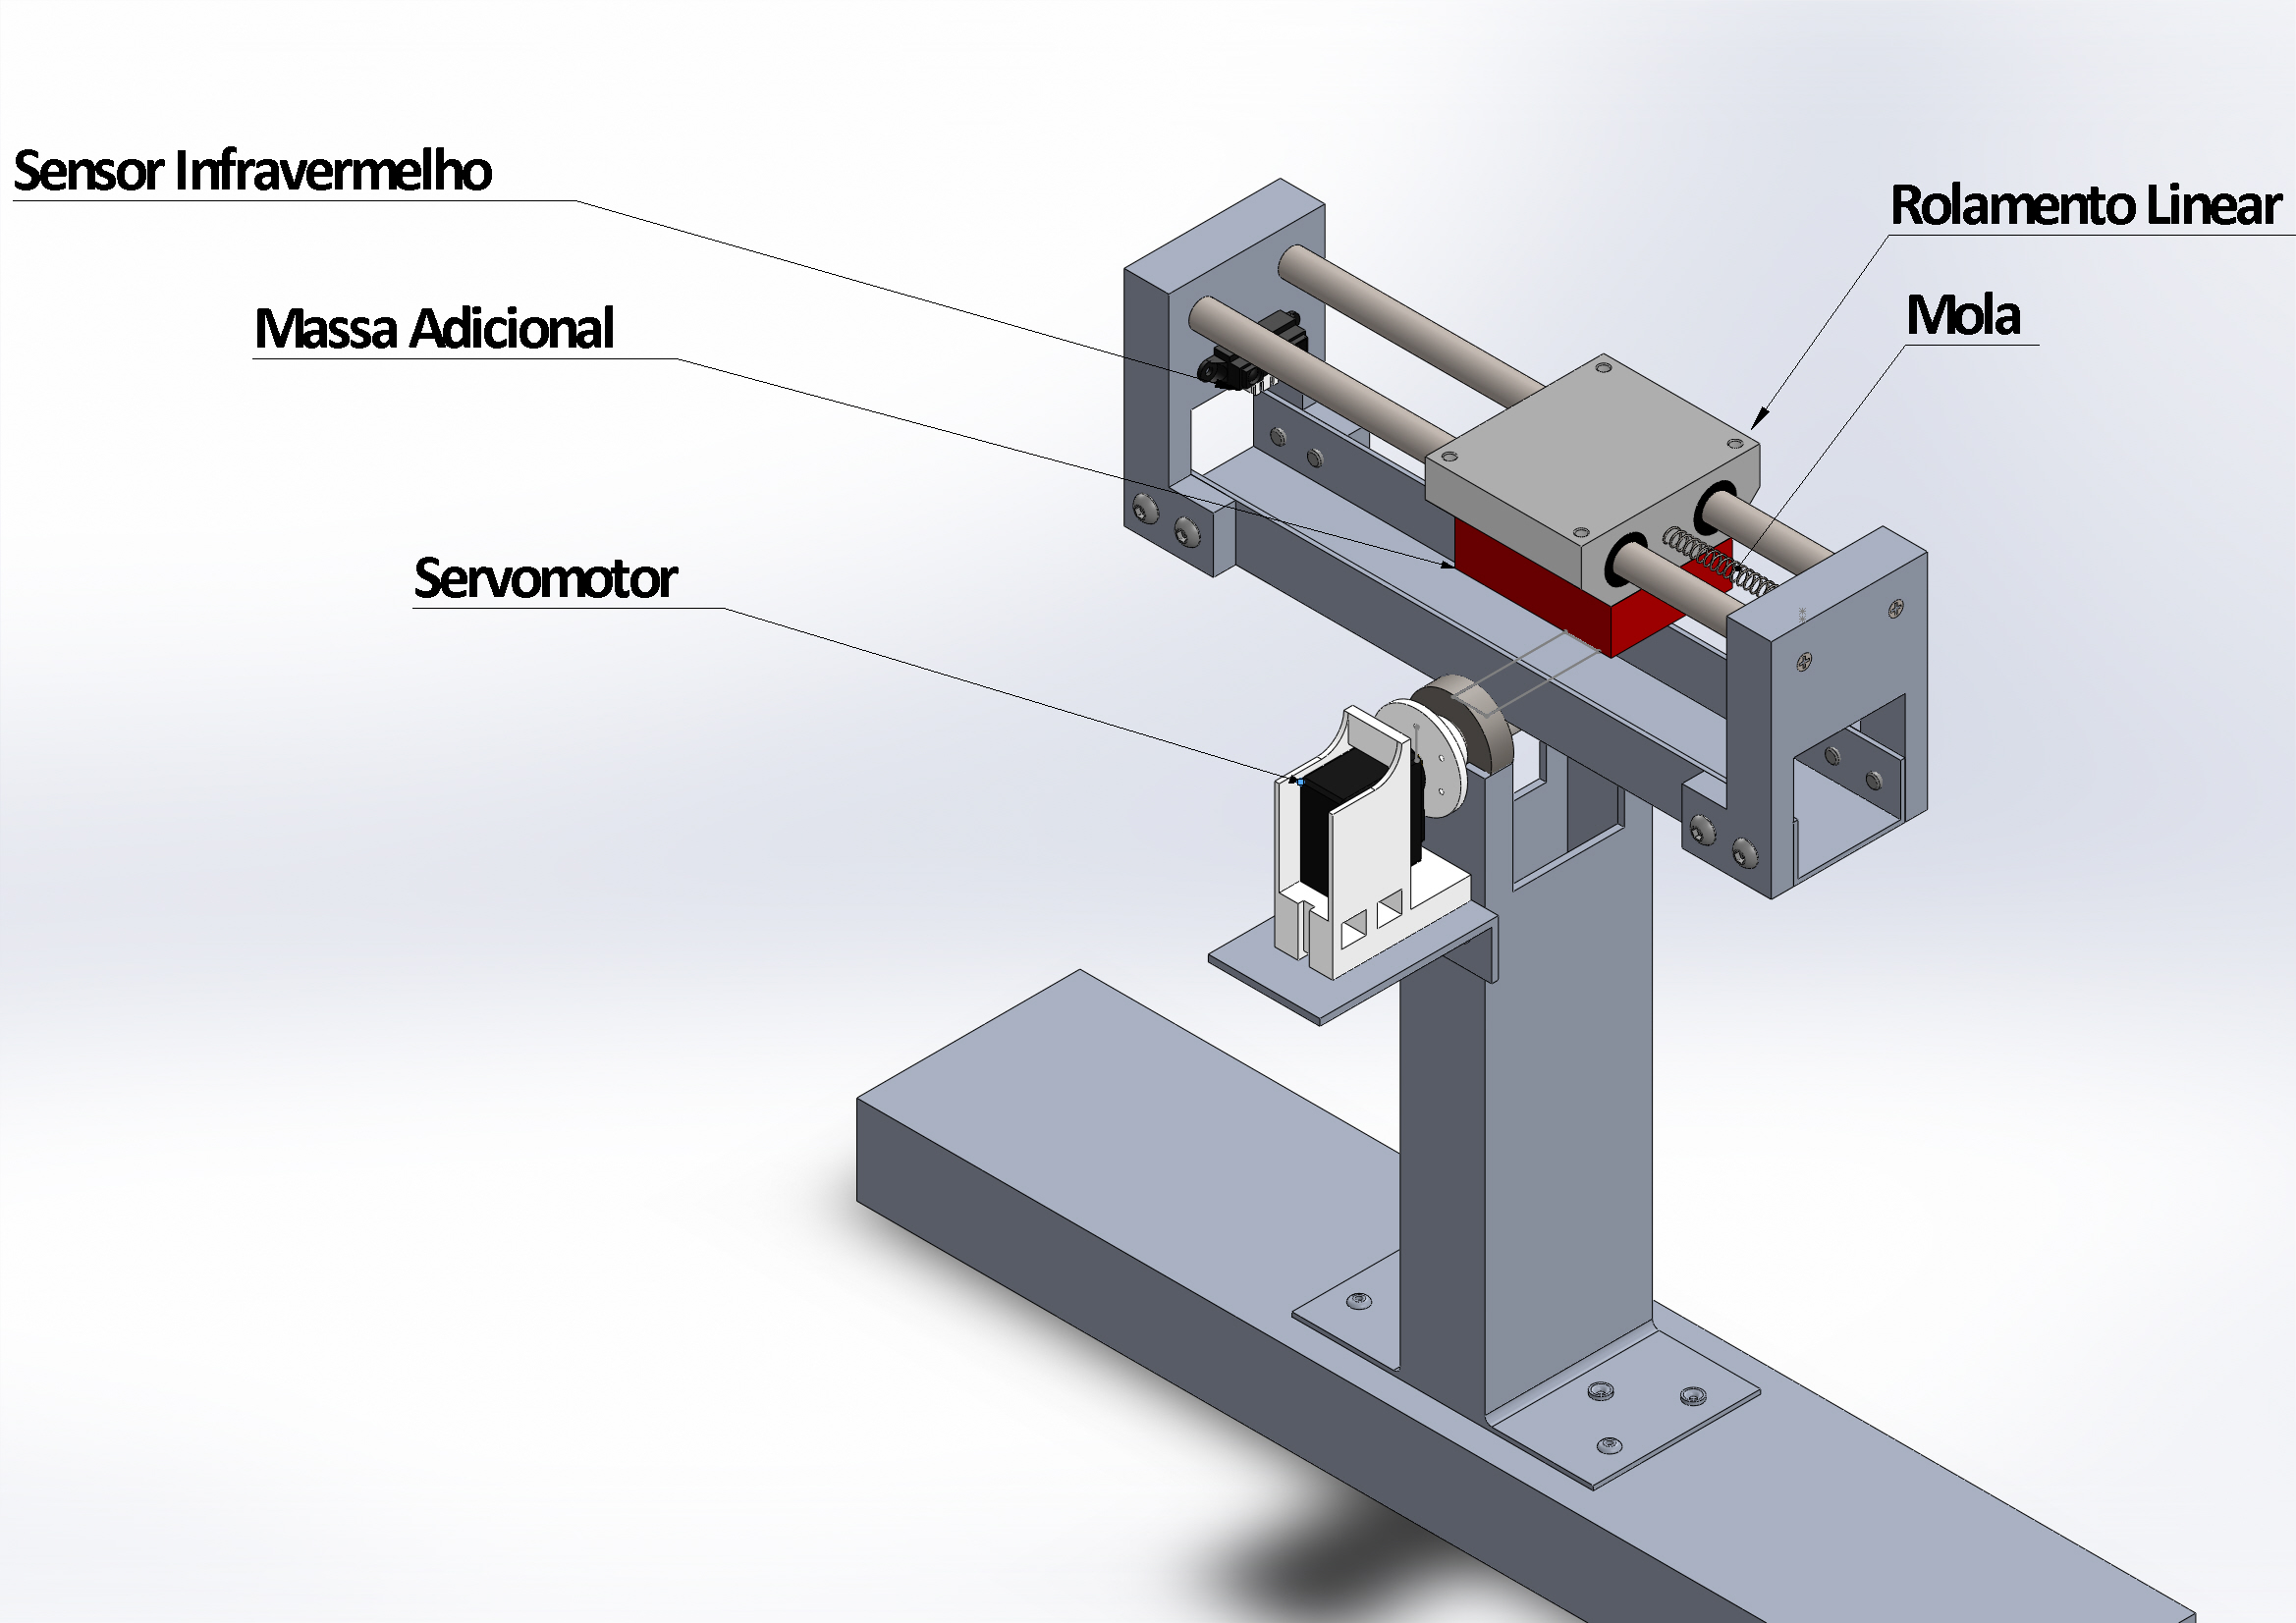
\includegraphics[width=0.8\linewidth]{imgs/planta}
		\caption{Sistema massa-mola em plano inclinado}%
		\label{fig:plant}
	\end{figure}
	\begin{figure}[H]
		\centering
		\captionsetup{justification=centering}
		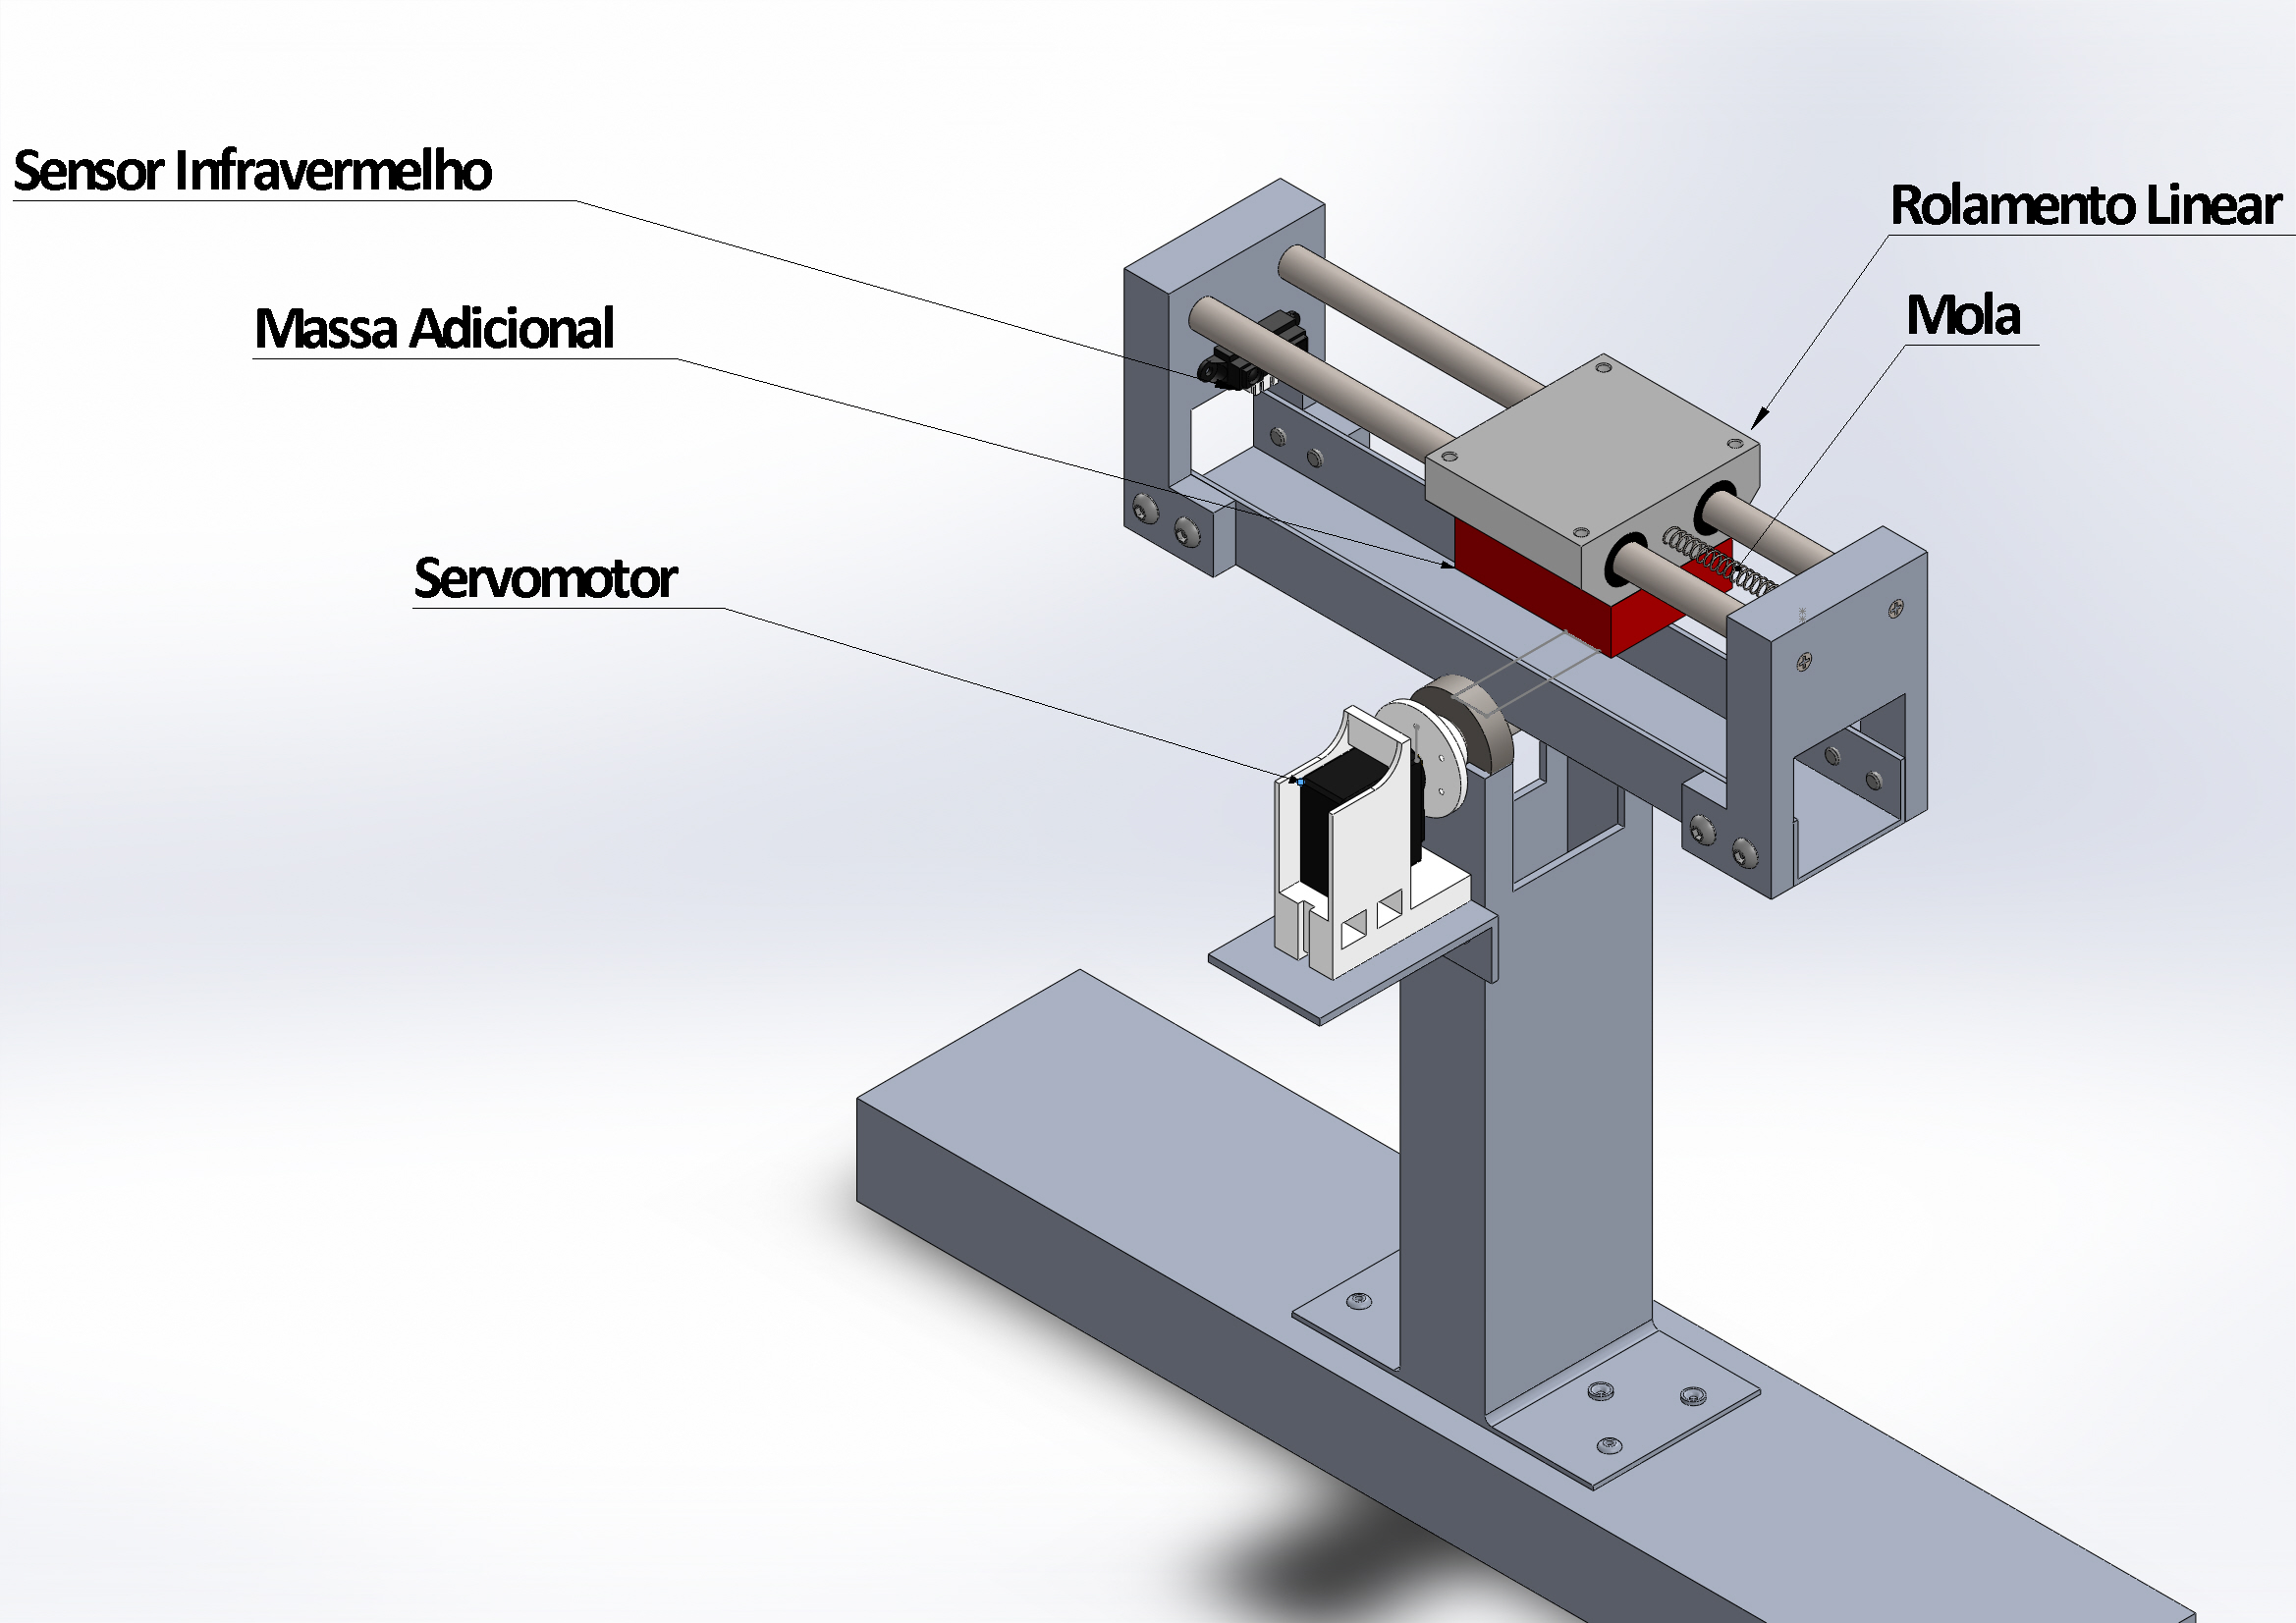
\includegraphics[width=0.8\linewidth]{imgs/planta}
		\caption{Sistema massa-mola em plano inclinado}%
		\label{fig:plant}
		\centering
		\captionsetup{justification=centering}
		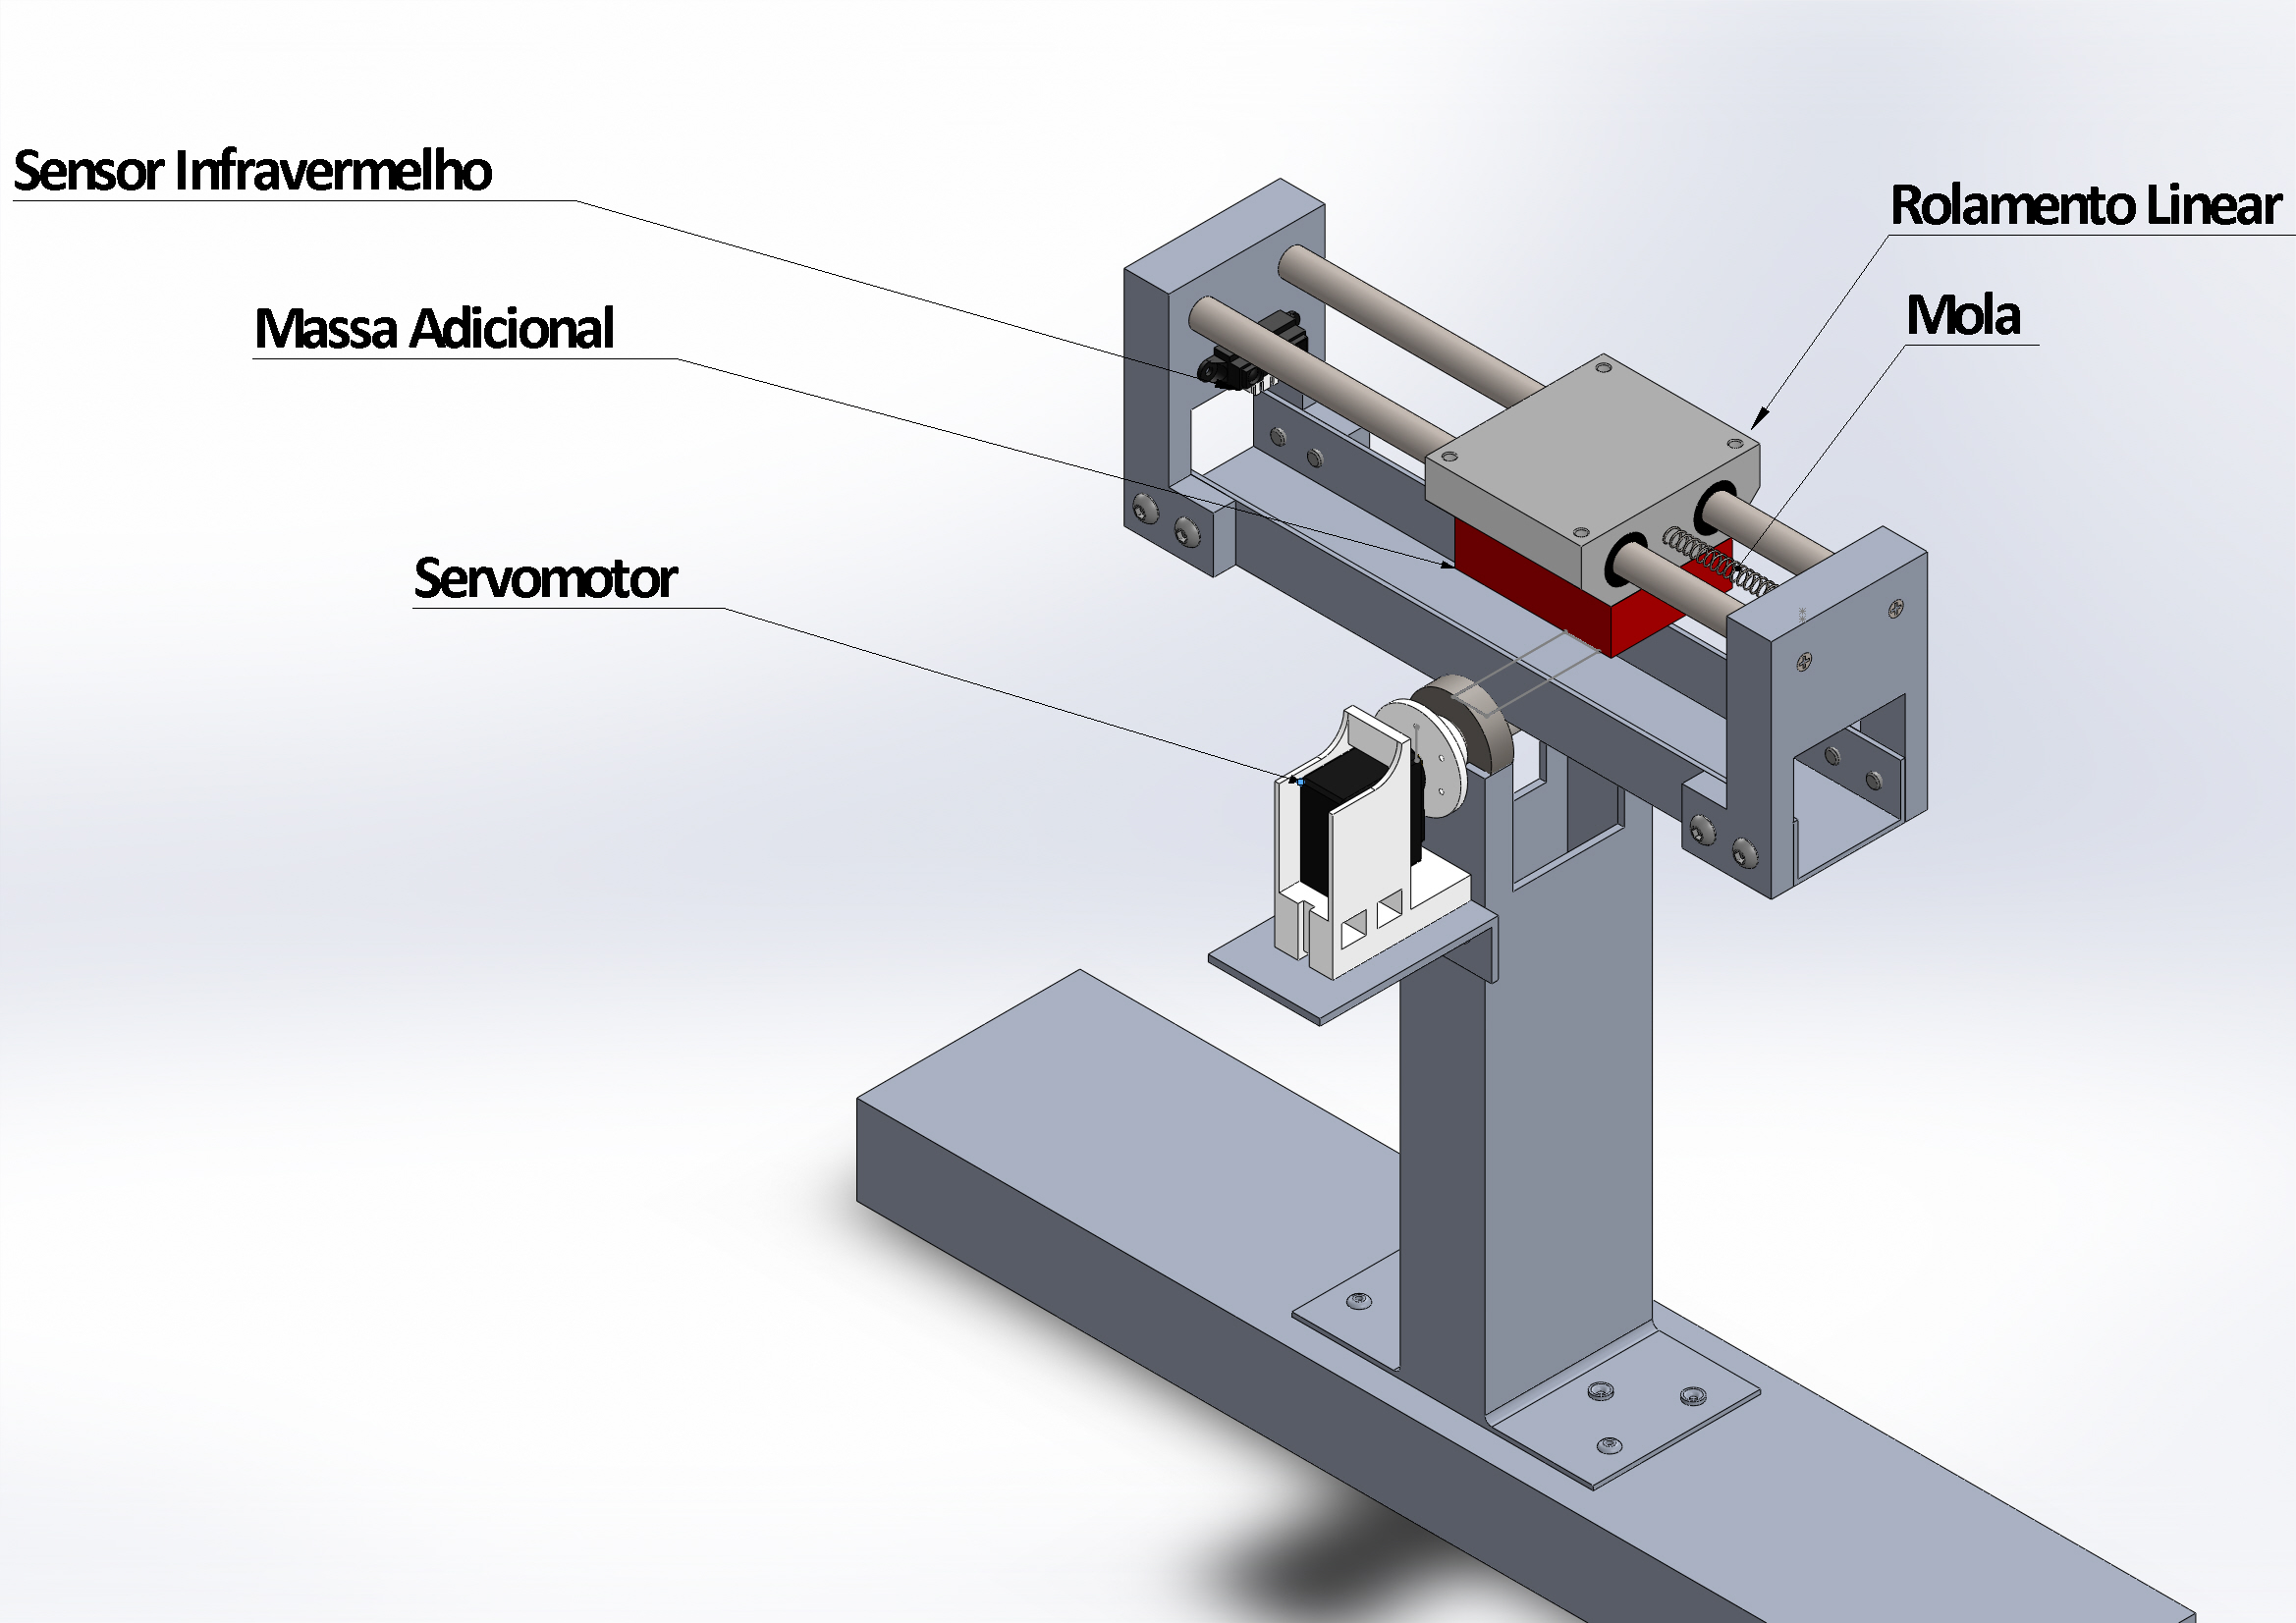
\includegraphics[width=0.8\linewidth]{imgs/planta}
		\caption{Sistema massa-mola em plano inclinado}%
		\label{fig:plant}
		\centering
		\captionsetup{justification=centering}
		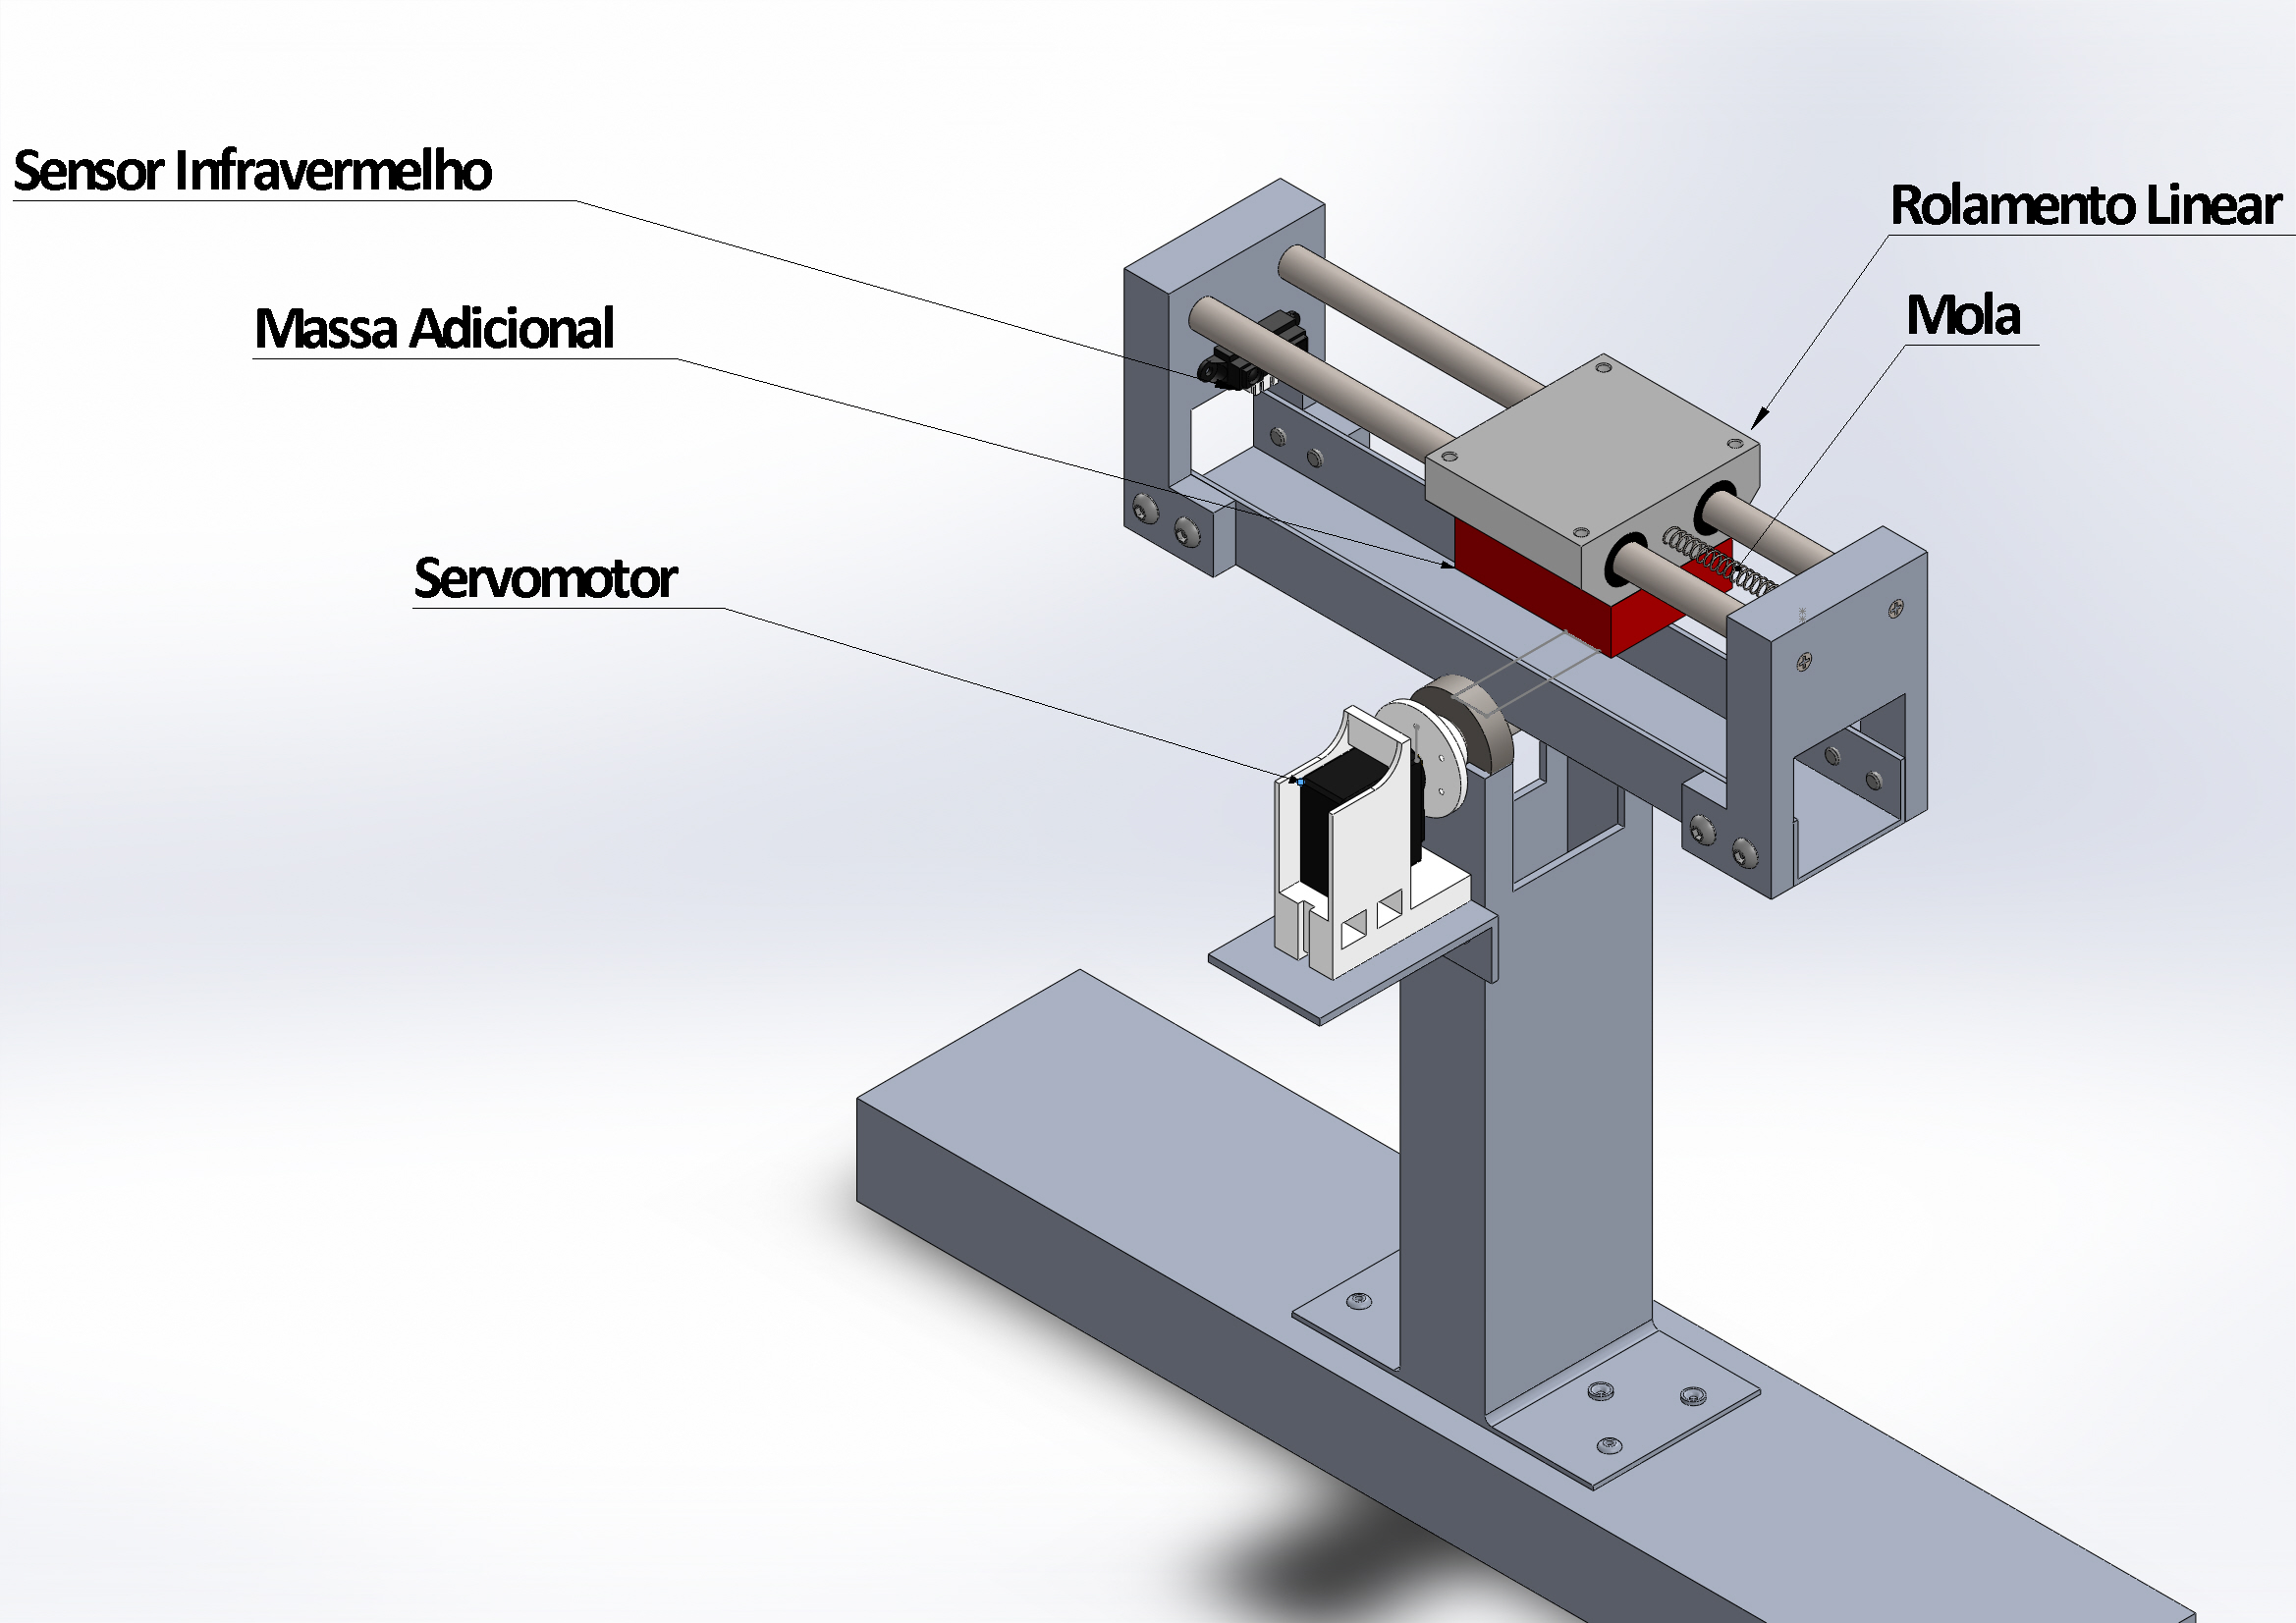
\includegraphics[width=0.8\linewidth]{imgs/planta}
		\caption{Sistema massa-mola em plano inclinado}%
		\label{fig:plant}
		\centering
		\captionsetup{justification=centering}
		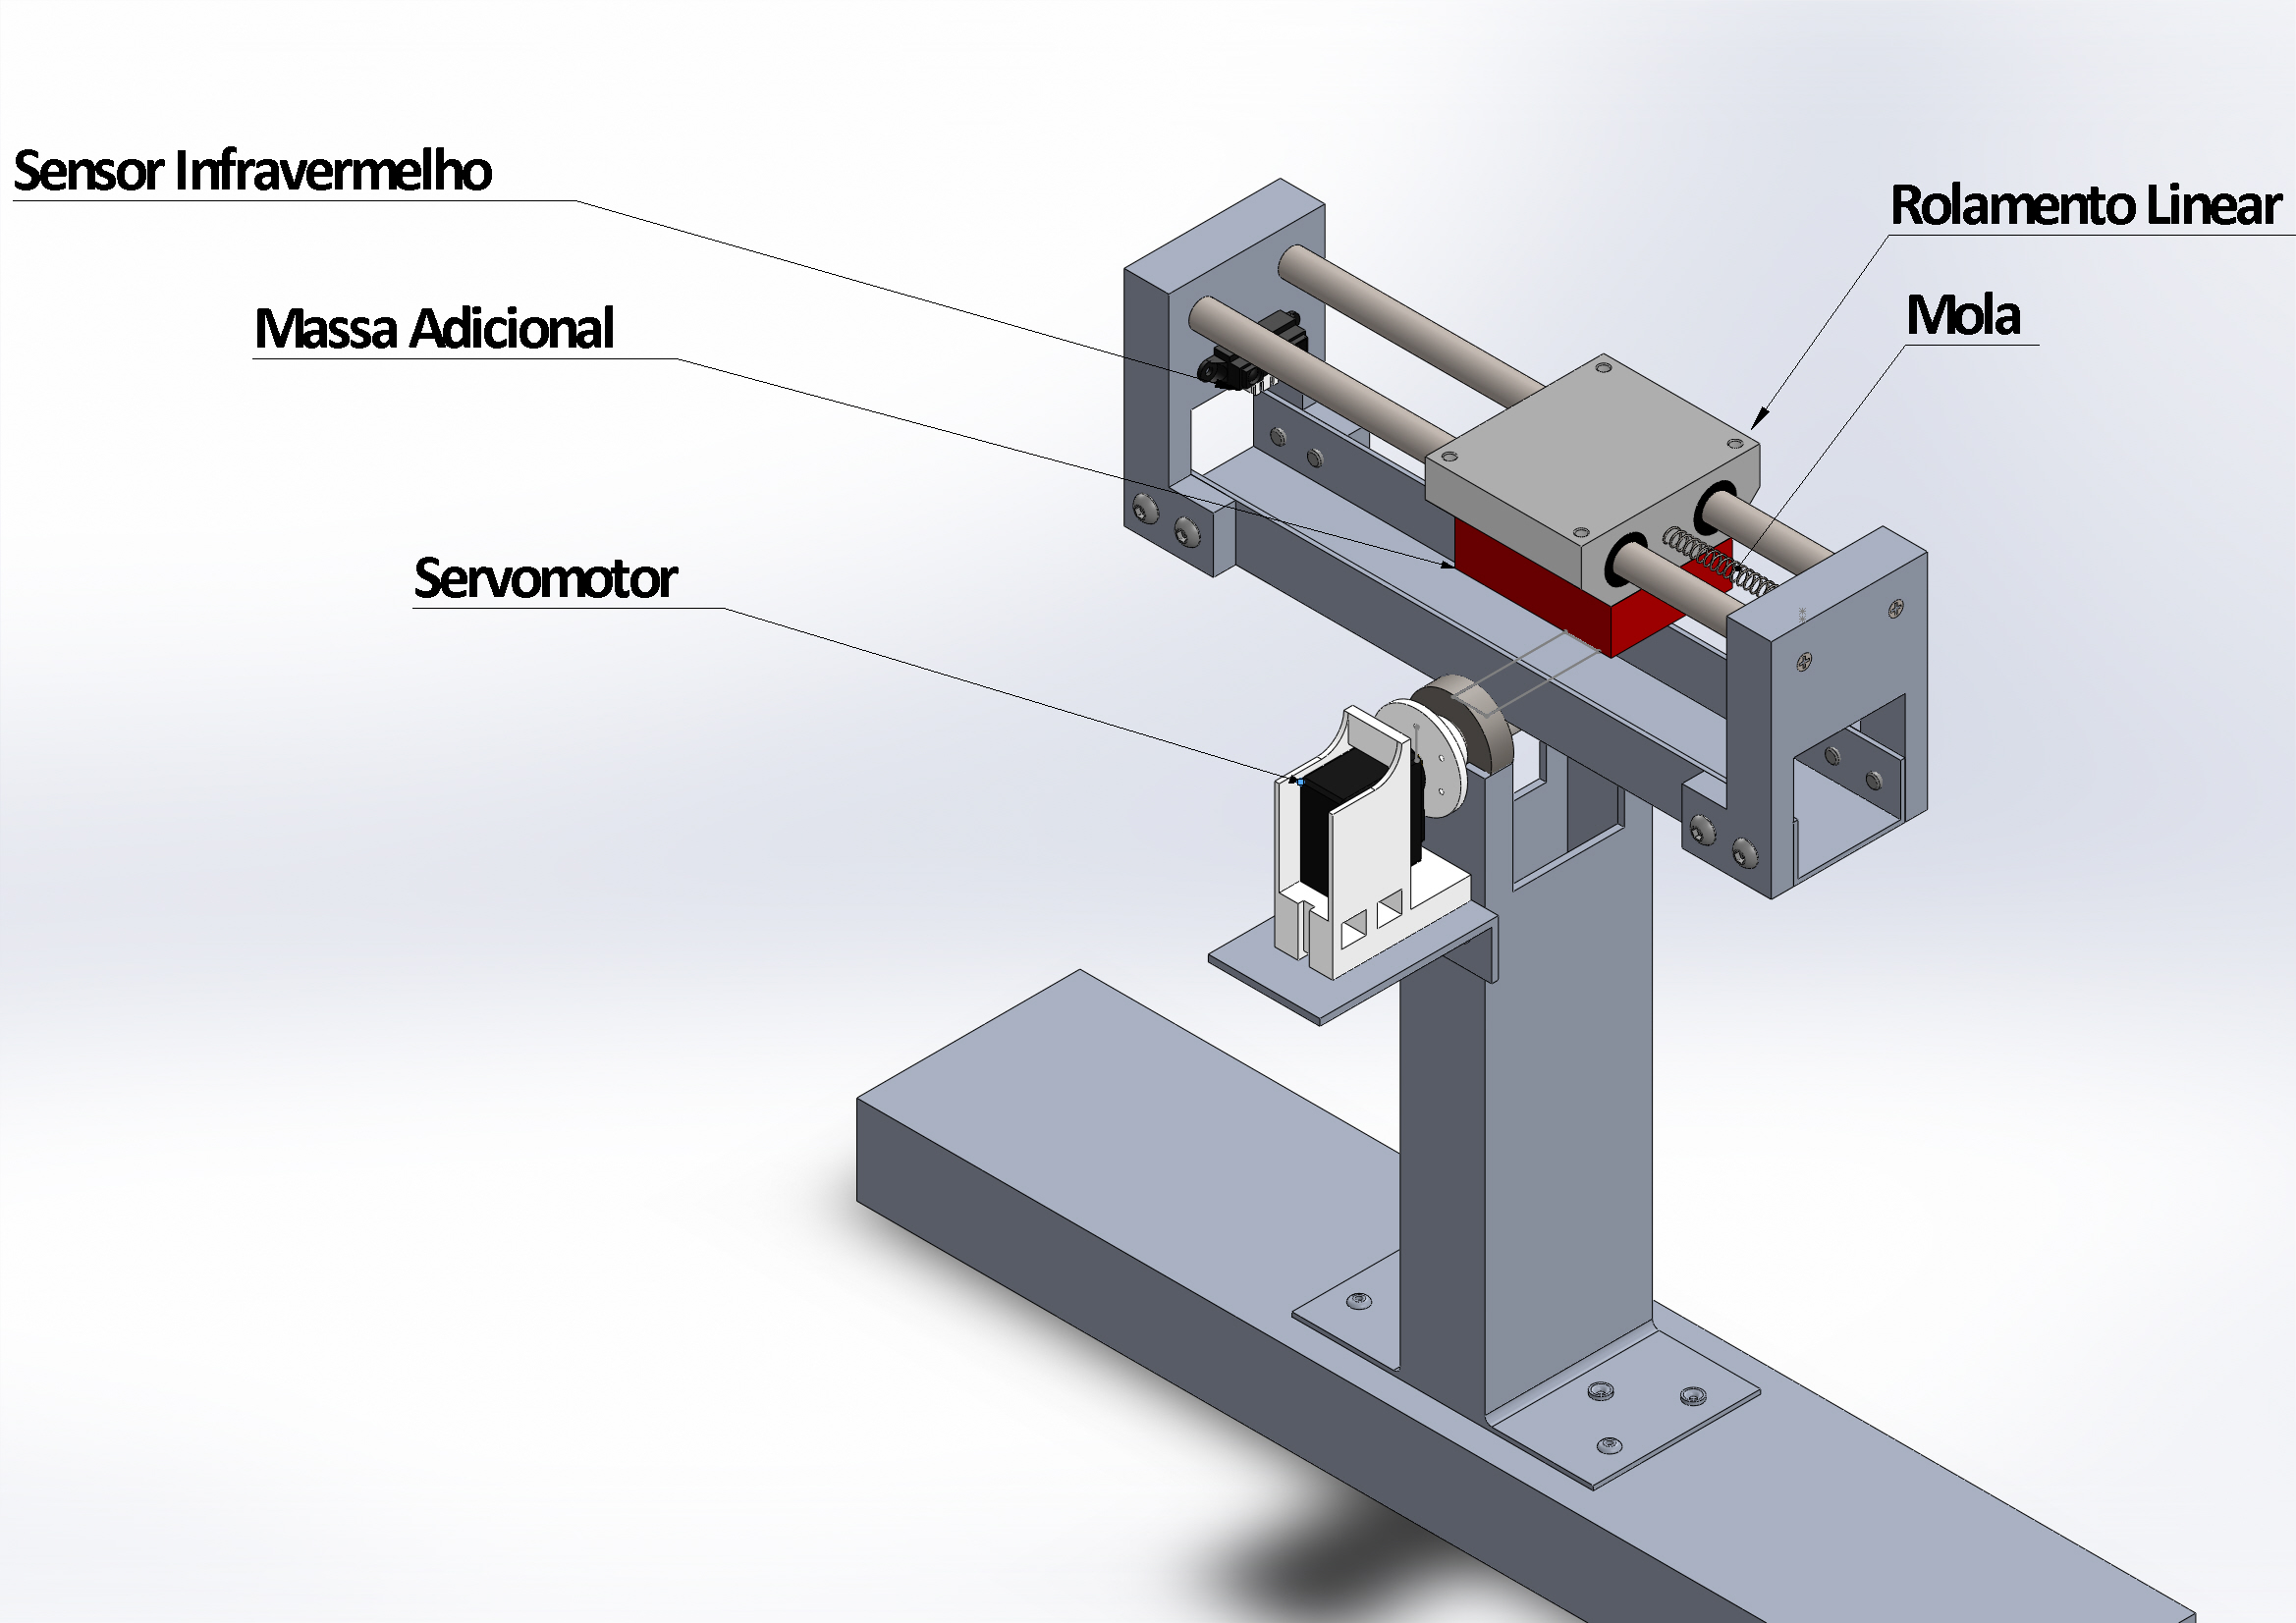
\includegraphics[width=0.8\linewidth]{imgs/planta}
		\caption{Sistema massa-mola em plano inclinado}%
		\label{fig:plant}
	\end{figure}
	\begin{table}[]
		\begin{tabular}{|cc|cc|cc|cc|cc|cc|cc|}
			\hline
			\multicolumn{2}{|c|}{Functions}      & \multicolumn{2}{c|}{Basic Blocks}   & \multicolumn{2}{c|}{Instructions}   & \multicolumn{2}{c|}{Loops}          & \multicolumn{2}{c|}{External Calls} & \multicolumn{2}{c|}{Direct Calls}   & \multicolumn{2}{c|}{\begin{tabular}[c]{@{}c@{}}Memory \\ Instructions\end{tabular}} \\ \hline
			\multicolumn{1}{|c|}{Before} & After & \multicolumn{1}{c|}{Before} & After & \multicolumn{1}{c|}{Before} & After & \multicolumn{1}{c|}{Before} & After & \multicolumn{1}{c|}{Before} & After & \multicolumn{1}{c|}{Before} & After & \multicolumn{1}{c|}{Before}                         & After                         \\ \hline
			&       &                             &       &                             &       &                             &       &                             &       &                             &       &                                                     &                               \\
			&       &                             &       &                             &       &                             &       &                             &       &                             &       &                                                     &                               \\ \hline
		\end{tabular}
	\end{table}
	\begin{table}[]
		\begin{tabular}{|cc|cc|cc|cc|cc|cc|cc|}
			\hline
			\multicolumn{2}{|c|}{Functions}      & \multicolumn{2}{c|}{Basic Blocks}   & \multicolumn{2}{c|}{Instructions}   & \multicolumn{2}{c|}{Loops}          & \multicolumn{2}{c|}{External Calls} & \multicolumn{2}{c|}{Direct Calls}   & \multicolumn{2}{c|}{\begin{tabular}[c]{@{}c@{}}Memory \\ Instructions\end{tabular}} \\ \hline
			\multicolumn{1}{|c|}{Before} & After & \multicolumn{1}{c|}{Before} & After & \multicolumn{1}{c|}{Before} & After & \multicolumn{1}{c|}{Before} & After & \multicolumn{1}{c|}{Before} & After & \multicolumn{1}{c|}{Before} & After & \multicolumn{1}{c|}{Before}                         & After                         \\ \hline
			&       &                             &       &                             &       &                             &       &                             &       &                             &       &                                                     &                               \\
			&       &                             &       &                             &       &                             &       &                             &       &                             &       &                                                     &                               \\ \hline
		\end{tabular}
	\end{table}
	\nocite{*}
	\printbibliography{}
\end{document}

